
\documentclass[12pt, reqno]{amsart}
\usepackage{amsmath, amsthm, amscd, amsfonts, amssymb, graphicx, color, esvect, subcaption, listings}
\usepackage[bookmarksnumbered, colorlinks, plainpages]{hyperref}

\definecolor{dkgreen}{rgb}{0,0.6,0}
\definecolor{gray}{rgb}{0.5,0.5,0.5}
\definecolor{mauve}{rgb}{0.58,0,0.82}

\lstset{frame=tb,
  language=Python,
  aboveskip=3mm,
  belowskip=3mm,
  showstringspaces=false,
  columns=flexible,
  basicstyle={\small\ttfamily},
  numbers=none,
  numberstyle=\tiny\color{gray},
  keywordstyle=\color{blue},
  commentstyle=\color{dkgreen},
  stringstyle=\color{mauve},
  breaklines=true,
  breakatwhitespace=true,
  tabsize=3
}

\textheight 22.5truecm \textwidth 14.5truecm
\setlength{\oddsidemargin}{0.35in}\setlength{\evensidemargin}{0.35in}
\setlength{\topmargin}{-.5cm}

\newtheorem{theorem}{Theorem}[section]
\newtheorem{lemma}[theorem]{Lemma}
\newtheorem{proposition}[theorem]{Proposition}
\newtheorem{corollary}[theorem]{Corollary}
\theoremstyle{definition}
\newtheorem{definition}[theorem]{Definition}
\newtheorem{example}[theorem]{Example}
\newtheorem{exercise}[theorem]{Exercise}
\newtheorem{conclusion}[theorem]{Conclusion}
\newtheorem{conjecture}[theorem]{Conjecture}
\newtheorem{criterion}[theorem]{Criterion}
\newtheorem{summary}[theorem]{Summary}
\newtheorem{axiom}[theorem]{Axiom}
\newtheorem{problem}[theorem]{Problem}
\theoremstyle{remark}
\newtheorem{remark}[theorem]{Remark}
\numberwithin{equation}{section}

\begin{document}
\setcounter{page}{1}

\title[Processing Digital Images using Singular Value Decomposition]{Processing Digital Images using Singular Value Decomposition}

\author[Y. Lakhotia, E. Pajaro]{Yuvraj Lakhotia$^1$ and Eden Pajaro$^2$}

\address{$^{1}$ Edison Academy Magnet School, Edison, NJ 08837, USA.}
\email{\textcolor[rgb]{0.00,0.00,0.84}{lakhotiay@mcmsnj.net}}

\address{$^{2}$ Edison Academy Magnet School, Edison, NJ 08837, USA.}
\email{\textcolor[rgb]{0.00,0.00,0.84}{pajaroe@mcmsnj.net}}

\keywords{Image processing, single value decomposition, linear algebra}

\begin{abstract}
In this paper, we explore the application of Singular Value Decomposition (SVD) in the processing of digital images. We delve into the mathematical principles of SVD and demonstrate its effectiveness in decomposing, compressing, and reconstructing images. The findings highlight the potential of SVD as a powerful tool for image analysis and enhancement in various digital imaging applications.
\end{abstract} \maketitle
\section{Introduction to Singular Value Decomposition}
\noindent Eugenio Beltrami (1835–1899) and Camille Jordan (1838–1921) independently discovered the SVD technique over a century ago \cite{Compton}. The development in the 1960s of practical methods for computing the SVD transformed the field of numerical linear algebra and established SVD as a staple in applied mathematics. In recent years, the SVD has become even more prominent due to a surge in increased computational memory and speed, as well as relevance to modern tasks. SVD involves decomposing a matrix into three constituent matrices, enabling a better understanding of the inherent structures within the data.

\begin{definition} We define the singular value decomposition of a matrix $A$ as
\begin{equation}\label{1.1}
A = U \Sigma V^\dagger
\end{equation}
\begin{enumerate}
    \item $A$: original $m \times n$ matrix with rank $r$ that is being factored
    \item $U$: $m \times m$ orthonormal matrix of left singular vectors
    \item $\Sigma$: $m \times n$ matrix with matrix $D$ in its upper-left corner, padded by 0's
    \item $D$: $r \times r$ diagonal matrix with first $r$ singular values of $A$ on main diagonal
    \item $V$: $n \times n$ orthonormal matrix of right singular vectors
\end{enumerate}
\end{definition}

\subsection{Prerequisites for SVD}
The foundations of SVD rest in a handful of basic linear algebra principles. Note that the factorization can be applied to any matrix, unlike the diagonalization method.

Below are a few important concepts that allow us to perform SVD \cite{Lay}\cite{Weisstein}.

\begin{enumerate}
\item \textbf{Rank:} often written as the $dim(Col A)$, it describes the number of linearly independent columns of $A$; the dimension of the column space of $A$.\\
\item \textbf{Orthogonal Matrix:} where $\vec{u} \cdot \vec{v}$ for all vector pairs in $Col(A)$ = 0. The vectors of an $m \times n$ orthogonal matrix spans $\mathbb{R}^n$, and $A^T$ = $A^{-1}$.\\
\item \textbf{Orthonormal Matrix:} an \textit{orthogonal matrix} $A$ where all $\vec{|v|}$ in $A$ = 1, where $\vec{v}$ refers to each vector in $Col(A)$.\\
\item \textbf{Symmetric Matrix:} a square matrix $A$ such that $A^T$ = $A$. Always orthogonally diagonalizable, such that there exists an orthogonal matrix $P$ and diagonal matrix $D$ where $A = PDP^{-1}$. Entries on the main diagonal are arbitrary, but other entries occur in pairs on opposite sides of the main diagonal. Eigenvectors from different eigenspaces are orthogonal.\\
\begin{equation*}
\text{Symmetric Matrices:}
\begin{bmatrix}
1 & 0\\
0 & -3
\end{bmatrix},
\begin{bmatrix}
0 & -1 & 0\\
-1 & 5 & 8\\
0 & 8 & -7    
\end{bmatrix},
\begin{bmatrix}
a & b & c\\
d & e & f\\
g & h & i
\end{bmatrix}
\end{equation*}
\item \textbf{Conjugate Transpose:} transpose of $A$ denoted $A^\dagger$, where each element is replaced with its complex conjugate. For real matrices, $A^T = A^\dagger$.\\
\end{enumerate}

\subsection{The Gram-Schmidt Process}
The construction of $U$, the $m \times m$ orthogonal matrix of left singular vectors of $A$, may require the extension of a set of vectors to an orthonormal basis for $\mathbb{R}^m$. This requires an understanding of orthogonal sets of vectors and the Gram-Schmidt process, an algorithm for finding an orthogonal or orthonormal basis for any nonzero subspace given a set of vectors that span the same subspace. It can be best explained by a visual example.
\begin{figure}[h]
    \centering
    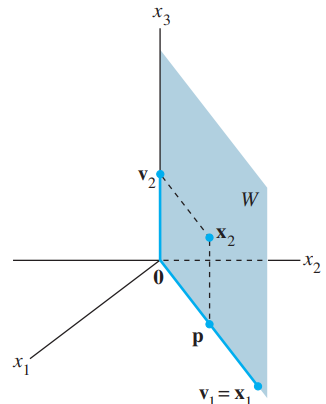
\includegraphics[width=0.3\linewidth]{img/gramschmidt.png}
    \caption{Construction of an orthogonal basis $\{v_1, v_2\}$ \cite{Lay}}
    \label{fig:gramschmidt}
\end{figure}
\begin{theorem}\label{theoGramSchmidt}
    Consider the subspace $W$, where $W = Span \{x_1, x_2\}$. To construct an orthogonal basis $\{v_1, v_2\}$ for $W$, understand that a vector can be decomposed into two components: its projection on an orthonormal set and the residual that is orthogonal to the given orthonormal set. We conclude that $Span\{v_1, v_2\} = Span \{x_1, x_2\} = W$.\\\\
    \noindent \normalfont{Keeping this in mind, the algorithm is generally intuitive. It involves keeping one vector from the original set to be a “stepping stone” and finding components of the other original vectors orthogonal to it using projections.}\\\\
    Let $v_1 = x_1$ and $p = proj_{x_1}x_2 = \frac{x_2 \cdot x_1}{x_1 \cdot x_1}x_1$. The component of $x_2 \perp x_1$ is $x_2 - p$. Thus, $v_2 = x_2 - p = x_2 - \frac{x_2 \cdot x_1}{x_1 \cdot x_1}x_1$. Given a basis $\{x_1,...,x_p\}$ for a nonzero subspace of $W$ of $\mathbb{R}^n$,
    \begin{align}\label{eqGramSchmidt}
        &v_1 = x_1\nonumber\\
        &v_2 = x_2 - \frac{x_2 \cdot v_1}{v_1 \cdot v_1}v_1\nonumber\\
        &v_3 = x_3 - \frac{x_3 \cdot v_1}{v_1 \cdot v_1}v_1 - \frac{x_3 \cdot v_2}{v_2 \cdot v_2}v_2\nonumber\\
        &\vdots\nonumber\\
        &v_p = x_p - \frac{x_p \cdot v_1}{v_1 \cdot v_1}v_1 - \frac{x_p \cdot v_2}{v_2 \cdot v_2}v_2 - ... - \frac{x_p \cdot v_{p-1}}{v_{p-1} \cdot v_{p-1}}v_{p-1}
    \end{align}
\end{theorem}

\subsection{Process for Calculating SVD}
Singular value decomposition is possible for any matrix, unlike diagonalization, which only works for some square matrices. Still, SVD is based on a property of ordinary diagonalization: the absolute value of the eigenvalues of a matrix measures the amount that matrix $A$ stretches or shrinks eigenvectors.\\\\
Recall that a symmetric matrix is orthogonally diagonalizable. There exists an orthogonal matrix $P$ and diagonal matrix $D$ where the symmetric matrix is equal to $PDP^{-1}$. For any $m \times n$ matrix $A$, $A^TA$ is a symmetric matrix and can therefore be orthogonally diagonalized. Note the eigenvectors of $A^TA$ form an orthonormal basis for $\mathbb{R}^n$ and the eigenvalues of $A^TA$ are nonnegative.\\\\
We can conclude $A$ is symmetric because $(A^TA)^T = A^TA^{TT} = A^TA$\\\\
The singular values of $A$ are the square roots of the positive eigenvalues of $A^TA$, denoted by $\sigma_1,...,\sigma_n$ and are arranged in decreasing order \cite{Fitzpatrick}. The singular values of $A$ are the lengths of the corresponding vectors $Av_1,...Av_n$ where $\{v_1...v_n\}$ is the set of eigenvectors of $A^TA$. $\sigma_1 = ||Av_1||$ where $\sigma_1 = \sqrt{\lambda_1}$ and $v_1$ is eigenvector corresponding to $\lambda_1$.
\begin{example}
    Constructing the SVD \eqref{1.1} of a matrix $A$ is divided into three steps. Consider an $m \times n$ matrix $A$ with rank $r = 1$ \cite{Serrano}.
    \begin{align*}
        A = 
        \begin{bmatrix}
            1 & -1\\
            -2 & 2\\
            2 & -2
        \end{bmatrix}
    \end{align*}
    \begin{enumerate}
        \item Find the orthogonal diagonalization of $A^TA$. Meaning, find the eigenvalues ($\lambda$) and correspeonding orthonormal eigenvectors of $A^TA$.
            \begin{equation}
                |A^TA - \lambda I| = \bigg|
                \begin{bmatrix}
                    9-\lambda & -9\\
                    -9 & 9-\lambda
                \end{bmatrix}\bigg| = 0, \\
                \lambda_1 = 18, \lambda_2 = 0
            \end{equation}
            It's important to order to the $\lambda$'s in decreasing order, as the singular values of $A$ must be in decreasing order.
            \begin{equation}
                \begin{split}
                    \lambda_1 = 18: 
                    \left[
                        \begin{array}{c|c}
                        A^TA - 18I & 0
                        \end{array}
                    \right]
                    \sim\
                    \left[
                        \begin{array}{c|c}
                        I & v_1
                        \end{array}
                    \right],
                    v_1 = \begin{bmatrix}
                        1/\sqrt{2}\\
                        -1\sqrt{2}
                    \end{bmatrix}\\
                    \lambda_2 = 0: 
                    \left[
                        \begin{array}{c|c}
                        A^TA - 0I & 0
                        \end{array}
                    \right]
                    \sim\
                    \left[
                        \begin{array}{c|c}
                        I & v_2
                        \end{array}
                    \right],
                    v_2 = \begin{bmatrix}
                        1/\sqrt{2}\\
                        1\sqrt{2}
                    \end{bmatrix}\\
                \end{split}
            \end{equation}
        \item Construct $V$ and $\Sigma$. $V$ is the $n \times n \; (2 \times 2)$  orthonormal matrix of right singular vectors from our calculated eigenvectors.
            \begin{equation}
                \begin{split}
                    V = \begin{bmatrix}
                        v_1 & v_2
                    \end{bmatrix}
                    = \begin{bmatrix}
                        1/\sqrt{2} & 1/\sqrt{2}\\
                        -1/\sqrt{2} & 1/\sqrt{2}
                    \end{bmatrix}\\
                    D = \begin{bmatrix}
                        \sqrt{\lambda_1} & 0\\
                        0 & \sqrt{\lambda_2}
                    \end{bmatrix}
                    = \begin{bmatrix}
                        3\sqrt{2} & 0\\
                        0 & 0
                    \end{bmatrix},
                    \Sigma = \begin{bmatrix}
                        3\sqrt{2} & 0\\
                        0 & 0\\
                        0 & 0
                    \end{bmatrix}
                \end{split}
            \end{equation}
        \item Construct $U$, an $m \times m \; (3 \times 3)$  orthonormal matrix of left singular vectors. The first $r$ columns of $U$ are the normalized vectors obtained from $Av_1...Av_r$. Since $r$ = 1 for $A$, the first column of $U$ is the normalized $Av_1$. Recall that $\sigma_1 = |Av_1|$.
            \begin{equation}
                u_1 = \frac{1}{\sigma_1}Av_1 
                = \frac{1}{3\sqrt{2}}Av_1
                = \begin{bmatrix}
                    1/3\\
                    -2/3\\
                    2/3
                \end{bmatrix}
            \end{equation}
        The remaining columns of $U$ are found by extending $\{u_1\}$ to an orthonormal basis for $\mathbb{R}^m$, in this case, $\mathbb{R}^3$. We need to find two orthogonal unit vectors, $u_2$ and $u_3$, that are $\perp$ $u_1$. The dot product of each vector $<x_1, x_2, x_3>$ and $u_1$ must be 0, satisfying $x_1 - 2x_2 + 2x_3 = 0$. We can find a basis for the solution, denoted by $w_1$ and $w_2$.
            \begin{equation}
                \begin{split}
                    w_1 = \begin{bmatrix}
                        2\\
                        1\\
                        0
                    \end{bmatrix},
                    w_2 = \begin{bmatrix}
                        -2\\
                        0\\
                        1
                    \end{bmatrix}
                \end{split}
            \end{equation}
        Now, $Span \{u_1, w_1, w_2\} = \mathbb{R}^m$ as they are $m$ linearly independent vectors in $\mathbb{R}^m$. However, $w_1$ and $w_2$ are $\perp$ $u_1$ but not to each other. To find an orthonormal basis for $\mathbb{R}^m$ given a set of vectors spanning $\mathbb{R}^m$, we use the Gram-Schmidt Process (\ref{theoGramSchmidt}) to obtain $u_2$ and $u_3$, and finally $U$.
            \begin{equation}
                \begin{split}
                    u_2 = \begin{bmatrix}
                        2/\sqrt{5}\\
                        1/\sqrt{5}\\
                        0
                    \end{bmatrix},
                    u_3 = \begin{bmatrix}
                        -2/3\sqrt{5}\\
                        4/3\sqrt{5}\\
                        5/3\sqrt{5}
                    \end{bmatrix}\\
                    U = \begin{bmatrix}
                        u_1 & u_2 & u_3
                    \end{bmatrix}
                    = \begin{bmatrix}
                        1/3 & 2/\sqrt{5} & -2/3\sqrt{5}\\
                        -2/3 & 2/\sqrt{5} & 4/3\sqrt{5}\\
                        2/3 & 0 & 5/3\sqrt{5}
                    \end{bmatrix}
                \end{split}
            \end{equation}
        \item Finally, set up the SVD factorization \eqref{1.1}.
            \begin{equation}
                \begin{bmatrix}
                    1 & -1\\
                    -2 & 2\\
                    2 & -2
                \end{bmatrix}
                = \begin{bmatrix}
                    1/3 & 2/\sqrt{5} & -2/3\sqrt{5}\\
                    -2/3 & 2/\sqrt{5} & 4/3\sqrt{5}\\
                    2/3 & 0 & 5/3\sqrt{5}
                \end{bmatrix}
                \begin{bmatrix}
                    3\sqrt{2} & 0\\
                    0 & 0\\
                    0 & 0
                \end{bmatrix}
                \begin{bmatrix}
                    1/\sqrt{2} & -1/\sqrt{2}\\
                    1/\sqrt{2} & 1/\sqrt{2}
                \end{bmatrix}\\
            \end{equation}
        This decomposition can be confirmed by using the NumPy library \cite{Lakhotia}.
\begin{lstlisting}
import numpy as np
from numpy.linalg import svd
A = [[1, -1], [-2, 2], [2, -2]]
U, S, V = svd(A)                                        # U, Sigma, V
#################################################################
# Output:
# U = [[-0.33333333  0.66666667 -0.66666667], [ 0.66666667  0.66666667  0.33333333], -0.66666667  0.33333333  0.66666667]]
# S = [4.24264069 0.        ]
# V = [[-0.70710678  0.70710678], [ 0.70710678  0.70710678]]
\end{lstlisting}
    \end{enumerate}
\end{example}
\section{Introduction to Digital Images}
\noindent Digital images are can be represented as a two-dimensional matrix of pixels, where the value of each pixel is commonly encoded using the popular RGB model.
\subsection{The RGB Model}
The popular RGB color model is an additive system that allows us to model any color in the visible spectrum as a triplet of integers ranging from 0-255 from wavelengths of primary colors red, green, and blue \cite{Zelazko}. This method is easy to apply to digital images, as digital displays are just rectangular grids of pixels. Each pixel's value is determined by the intensity of red, green, and blue colors for that location blended together to generate a certain shade \cite{Devi}. In this way, we can represent an entire display or image with three grids.

\begin{figure}[h]
    \begin{subfigure}{0.58\linewidth}
        \centering
        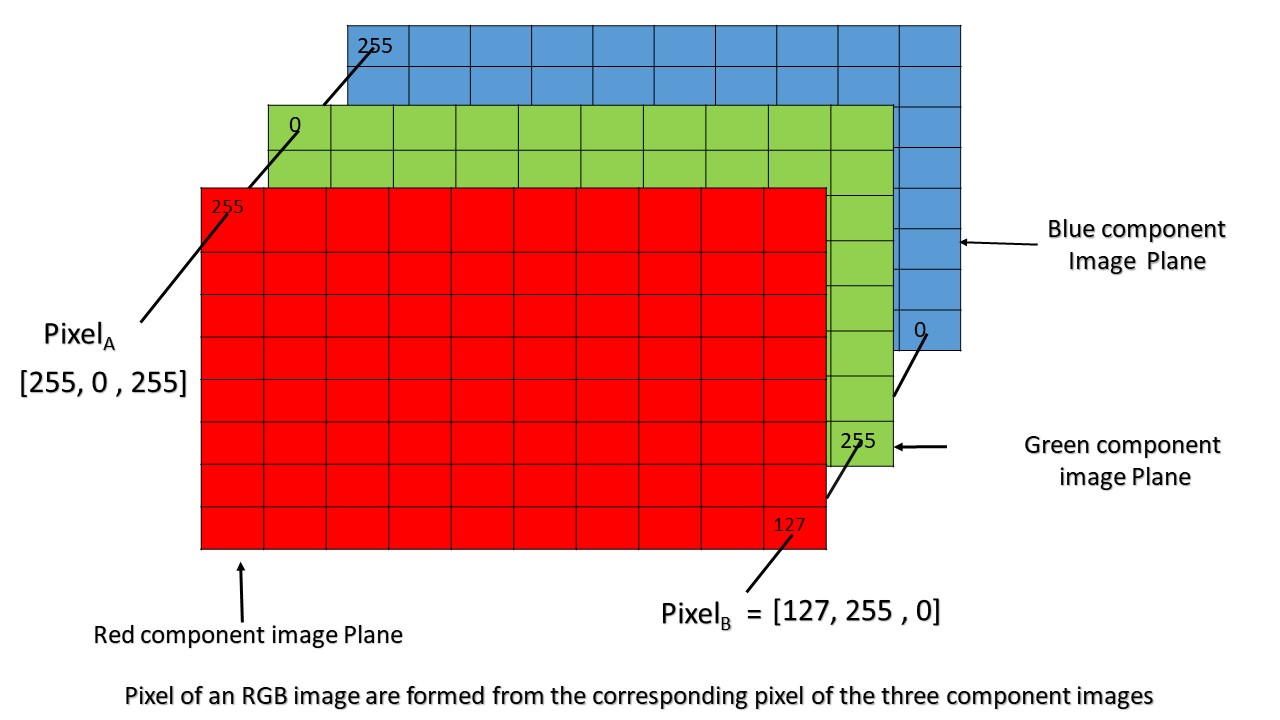
\includegraphics[height=5cm]{img/rgb1.jpeg} 
        \caption{RGB Image Planes}
        \label{fig:rgbim1}
    \end{subfigure}
    \begin{subfigure}{0.41\linewidth}
        \centering
        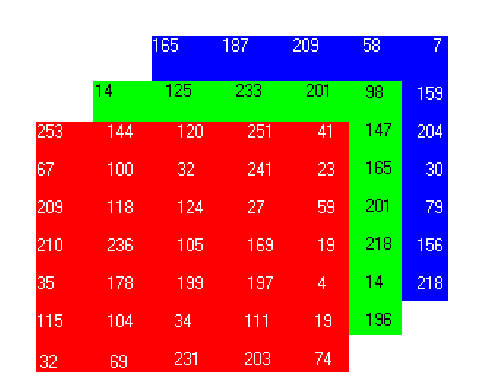
\includegraphics[height=5cm]{img/rgb2.png}
        \caption{Sample RGB Values}
        \label{fig:rgbim2}
    \end{subfigure}
    \caption{RGB Color Channels}
    \label{fig:rgb}
\end{figure}

\noindent As seen in Figure \ref{fig:rgb}, each color channel—red, green, blue—in the RGB spectrum is assigned its own grid of values that specify the intensity that respective color in the final image. The final image is generated by combining each channel's value to generate a specific color. For reference, black can be modeled as $(0, 0, 0)$ and white can be modeled as $(255, 255, 255)$.

\begin{example}
We can now experiment with this ourselves by processing an existing RGB image \cite{Lakhotia} and separating it into its three RGB color channels.
\begin{figure}[h]
    \centering
    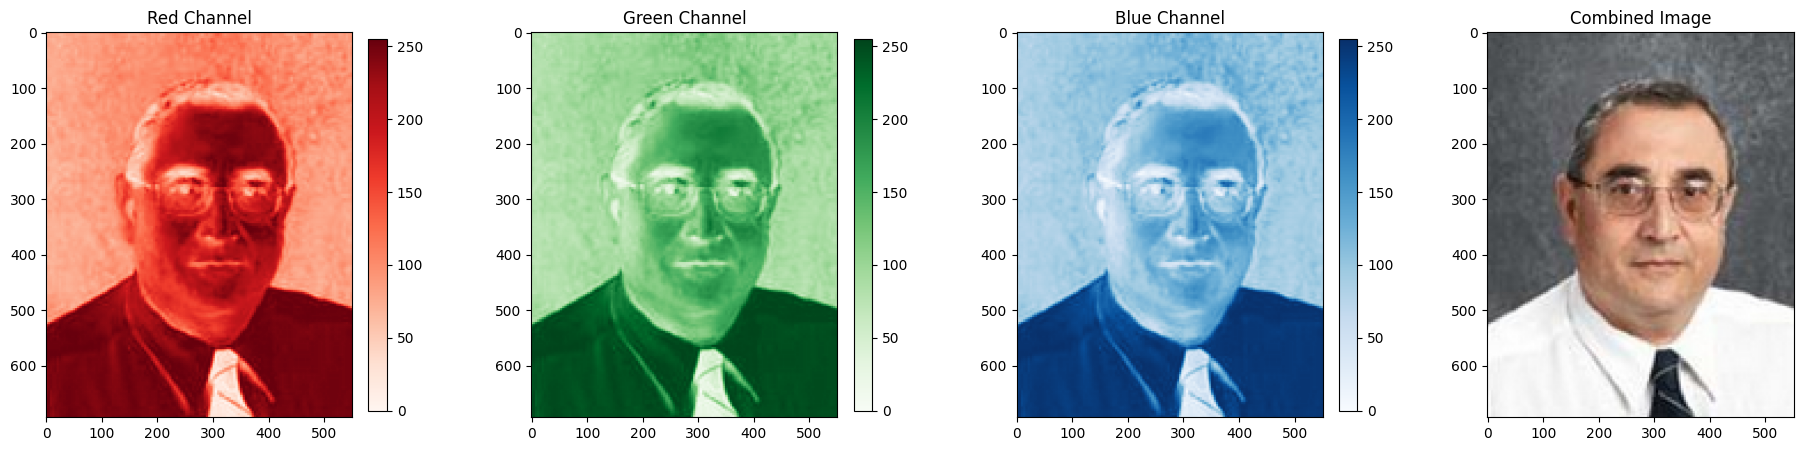
\includegraphics[width=\linewidth]{img/rgbchannels.png}
    \caption{RGB Channels of a 551 $\times$ 693 image of Mr. E. Paterno}
    \label{fig:rgbarray}
\end{figure}
\end{example}

\subsection{Storing Digital Images}
Image files require disk space to be stored. Depending on the resolution, quality, and format of the image, it may require a few kilobytes (kB) or several megabytes (MB) to persist an image file to the disk \cite{BBC}. In the RGB model, each pixel requires three bytes of storage—one for each color channel. This is because each byte holds eight bits of information, allowing it to express $2^8 = 256$ distinct integers: 0-255.
\begin{example}
    Recalling that each pixel in an RGB image takes up three bytes, and that an image with resolution $m \times n$ has $m \times n$ pixels, we can roughly estimate the size, in bytes, of an RGB image given its resolution. This relationship $(size = 3mn)$ can be visualized in Figure \ref{fig:imgsizes} to show the importance of minimizing file size to save disk space \cite{Lakhotia}.
    \begin{figure}[h]
        \centering
        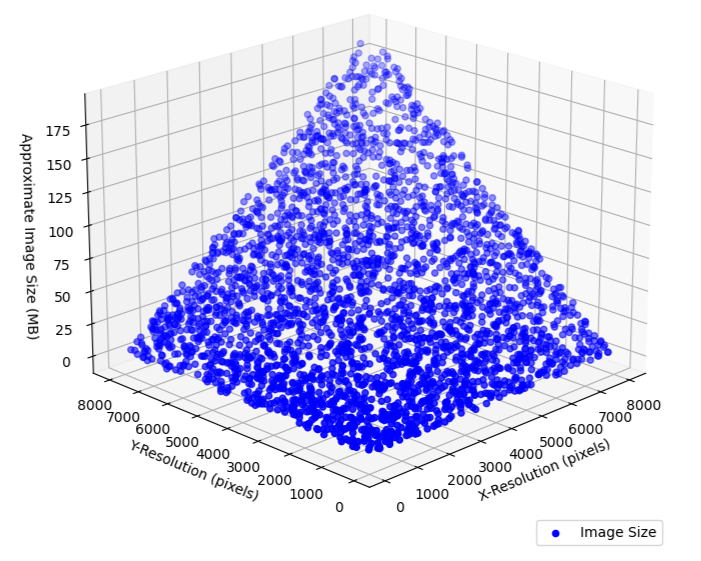
\includegraphics[width=0.5\linewidth]{img/imagesizes.png}
        \caption{Storage (MB) required for each of 3,000 random images}
        \label{fig:imgsizes}
    \end{figure}
\end{example}

\section{Applying SVD to Compress Digital Images}
\noindent We've discussed how digital images are represented by a grid of color values for each pixel. To better fit into our discussion of the use of linear algebra in image processing, we'll start referring to this grid as a matrix. Recall that SVD can be performed on any matrix—so all digital images can be factored using SVD.\\ 
\subsection{Low-Rank Matrix Approximations}
An important application of SVD is making approximations. Before we take on the greater topic of image processing, it’s important to understand how the organization of the matrices that comprise SVD reveals the important features of the original matrix $A$. $A = U \Sigma V^\dagger$ where $\Sigma$ contains a diagonal matrix of decreasing singular values. Thus, the SVD of $A$ can be expression as the following sum of matrices \cite{Serrano}.
\begin{equation}\label{eqlowrank}
    A = \sigma_1 u_1 v_1^\dagger + \sigma_2 u_2 v_2^\dagger + ... \sigma_n u_n v_n^\dagger
\end{equation}
\begin{figure}[h]
    \centering
    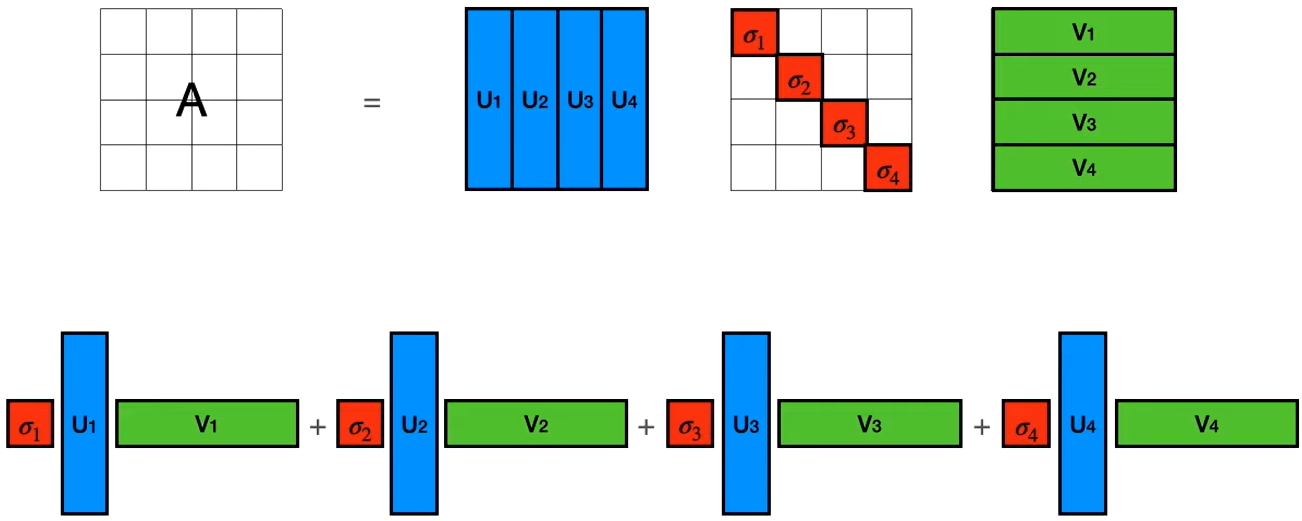
\includegraphics[width=0.6\linewidth]{img/lowrankapprox.png}
    \caption{Separating the SVD of $A$ into a sum of matrices}
    \label{fig:lowrank}
\end{figure}\\
To derive an approximation for $A$ from its SVD, recall that singular values are arranged in decreasing order. Each successive term in the sum of matrices creates smaller, more precise changes than to its predecessor. $A$ can be approximated by dropping or truncating the “least important,” less influential terms, starting with the last term.
\begin{example}
    Consider a $3 \times 2$ matrix $A$ and its SVD factorized form.
    \begin{equation}
        A = \begin{bmatrix}
            1 & 2\\
            3 & 1\\
            2 & 3\\
        \end{bmatrix}
        = \begin{bmatrix}
            3/5\sqrt{2} & -1\sqrt{6} & 7/5\sqrt{3}\\
            4/5\sqrt{2} & -2\sqrt{6} & 1/5\sqrt{3}\\
            -1/\sqrt{2} & 1\sqrt{6} & -1/\sqrt{3}
            % \frac{3}{5\sqrt{2}} & \frac{-1}{\sqrt{6}} & \frac{7}{5\sqrt{3}}\\
            % \frac{4}{5\sqrt{2}} & \frac{-2}{\sqrt{6}} & \frac{1}{5\sqrt{3}}\\
            % \frac{-1}{\sqrt{2}} & \frac{1}{\sqrt{6}} & \frac{-1}{\sqrt{3}}
        \end{bmatrix}
        \begin{bmatrix}
            5 & 0\\
            0 & \sqrt{3}\\
            0 & 0
        \end{bmatrix}
        \begin{bmatrix}
            1\sqrt{2} & 1/\sqrt{2}\\
            -1\sqrt{2} & 1/\sqrt{2}
        \end{bmatrix}
    \end{equation}\\
    This SVD can also be expressed as $A = \sigma_1 u_1 v_1^\dagger + \sigma_2 u_2 v_2^\dagger$. The last term, with its coefficient being the smallest singular value, can be dropped or truncated to approximate $A$. This is known as a rank-$1$ approximation, and we can generally term these as rank-$k$ approximations which use the first \textit{k} singular values/terms.
    \begin{equation}
        A \approx A_1 = \sigma_1 u_1 v_1^\dagger = 5
        \begin{bmatrix}
            3/5\sqrt{2}\\
            4/5\sqrt{2}\\
            1/\sqrt{2}
        \end{bmatrix}
        \begin{bmatrix}
            1/\sqrt{2}\\
            1/\sqrt{2}
        \end{bmatrix}
        = \begin{bmatrix}
            1.5 & 1.5\\
            2 & 2\\
            2.5 & 2.5
        \end{bmatrix}
        \approx
        \begin{bmatrix}
            1 & 2\\
            3 & 1\\
            2 & 3\\
        \end{bmatrix}
    \end{equation}
This approximation is far from the original matrix because $A$ is relatively small matrix with rank 2. In real-world applications, matrices may have tens of thousands of elements. In those cases, such as matrices representing digital images, the rank of the matrix may be approaching the thousands and removing a handful of the least influential terms would result in a more impressive approximation.
\end{example}
\subsection{Grayscale Image Compression}
In a grayscale image, we can represent each pixel as a 0 or 1, which is black and white, respectively. With only two possible states (on or off) for each pixel, the matrices for grayscale images are fairly simple. Still, they are  effective in illustrating the outputs of rank-$k$ approximations. 
\begin{example}
    Let us look at this $6 \times 7$ image matrix that represents a heart.
    \begin{equation}
        A = \begin{bmatrix}
            0 & 1 & 1 & 0 & 1 & 1 & 0 \\
            1 & 1 & 1 & 1 & 1 & 1 & 1 \\
            1 & 1 & 1 & 1 & 1 & 1 & 1 \\
            0 & 1 & 1 & 1 & 1 & 1 & 0 \\
            0 & 0 & 1 & 1 & 1 & 0 & 0 \\
            0 & 0 & 0 & 1 & 0 & 0 & 0
        \end{bmatrix}
    \end{equation}
    \begin{figure}[h]
        \centering
        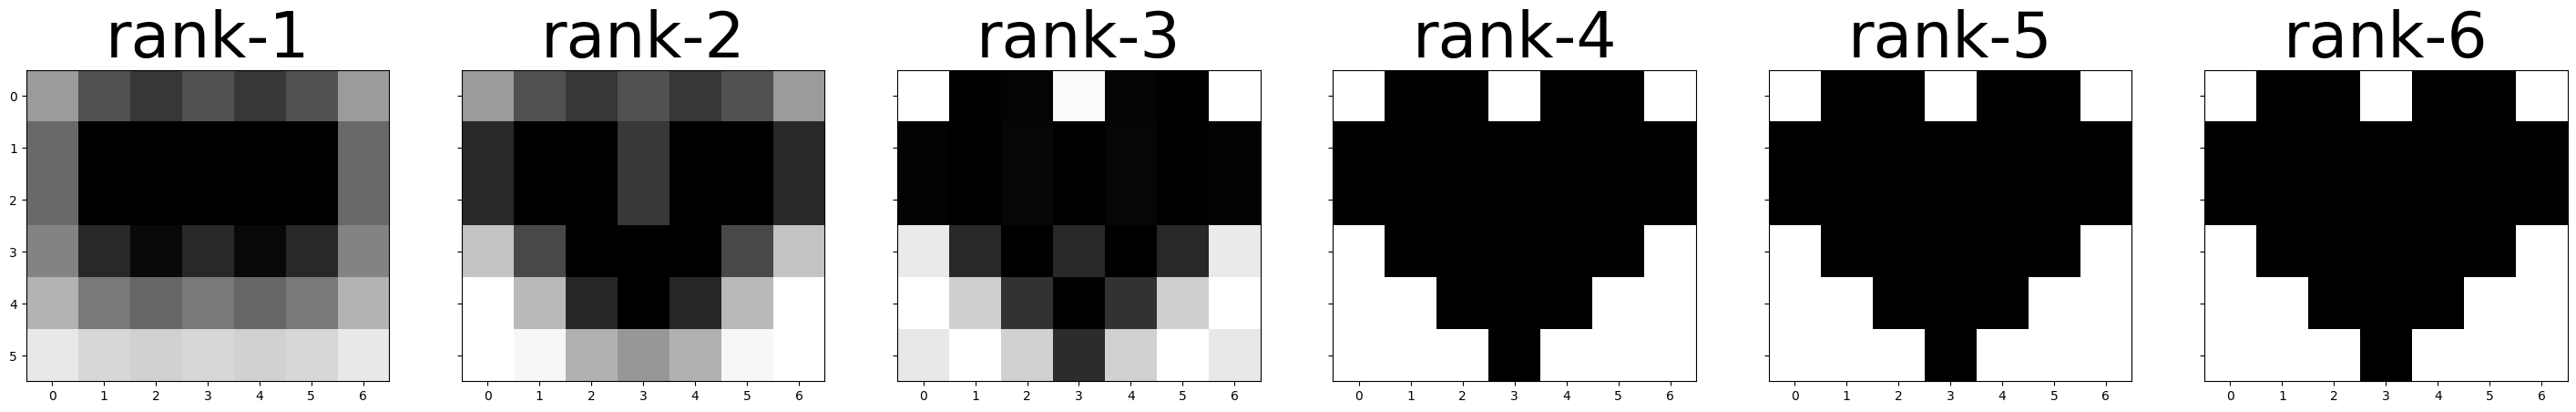
\includegraphics[width=\linewidth]{img/grayscaleheart.png}
        \caption{Rank-$k$ approximations of $A$, where rank(A) = 6}
        \label{fig:heartgrayscale}
    \end{figure}\\
    Note how the lower-rank approximations of A created a rough sketch of the heart and higher-rank approximations simply made finer tunings until we restored the original image and approached $k = r$. Also note how the rank-4 to rank-6 approximations are indistinguisable to the human eye—although there are extremely small differences at the pixel-level, we can say that they're "good enough" for now.\\\\
    We can choose to store the the rank-4 image instead of the original and truncate the last 2 terms, saving storage that would have been occupied by $\sigma_5 u_5 v_5^\dagger + \sigma_6 u_6 v_6^\dagger$. The storage saved by truncating terms with minimal impact will become more apparent with larger files.
\end{example}
\subsection{RGB Image Compression}
Recall that an RGB image is represented by three color channels, each modeled by a matrix. SVD can be performed on each matrix, allowing each color channel to be factored and approximated. The factorizations can then be combined to visualize a rank-$k$ approximation for the original image. This approximation takes up less space than the original image while retaining its likeness.
\begin{example}
    We find a similar heart in color! $R, G, B$ channels, respectively:
    \begin{equation*}
        \fontsize{6pt}{1pt}
        \begin{bmatrix}
            0 & 255 & 255 & 0 & 255 & 255 & 0 \\
            255 & 221 & 221 & 255 & 221 & 221 & 255 \\
            255 & 221 & 221 & 190 & 221 & 221 & 255 \\
            0 & 255 & 190 & 190 & 190 & 255 & 0 \\
            0 & 0 & 255 & 190 & 255 & 0 & 0 \\
            0 & 0 & 0 & 255 & 0 & 0 & 0
        \end{bmatrix},
         \begin{bmatrix}
            0 & 0 & 0 & 0 & 0 & 0 & 0 \\
            0 & 70 & 70 & 0 & 70 & 70 & 0 \\
            0 & 70 & 70 & 70 & 70 & 70 & 0 \\
            0 & 0 & 70 & 70 & 70 & 0 & 0 \\
            0 & 0 & 0 & 70 & 0 & 0 & 0 \\
            0 & 0 & 0 & 0 & 0 & 0 & 0\\
        \end{bmatrix},
         \begin{bmatrix}
            0 & 0 & 0 & 0 & 0 & 0 & 0 \\
            0 & 200 & 200 & 0 & 200 & 200 & 0 \\
            0 & 200 & 200 & 221 & 200 & 200 & 0 \\
            0 & 0 & 221 & 221 & 221 & 0 & 0 \\
            0 & 0 & 0 & 221 & 0 & 0 & 0 \\
            0 & 0 & 0 & 0 & 0 & 0 & 0\\
        \end{bmatrix}
    \end{equation*}
    \begin{figure}[h]
        \centering
        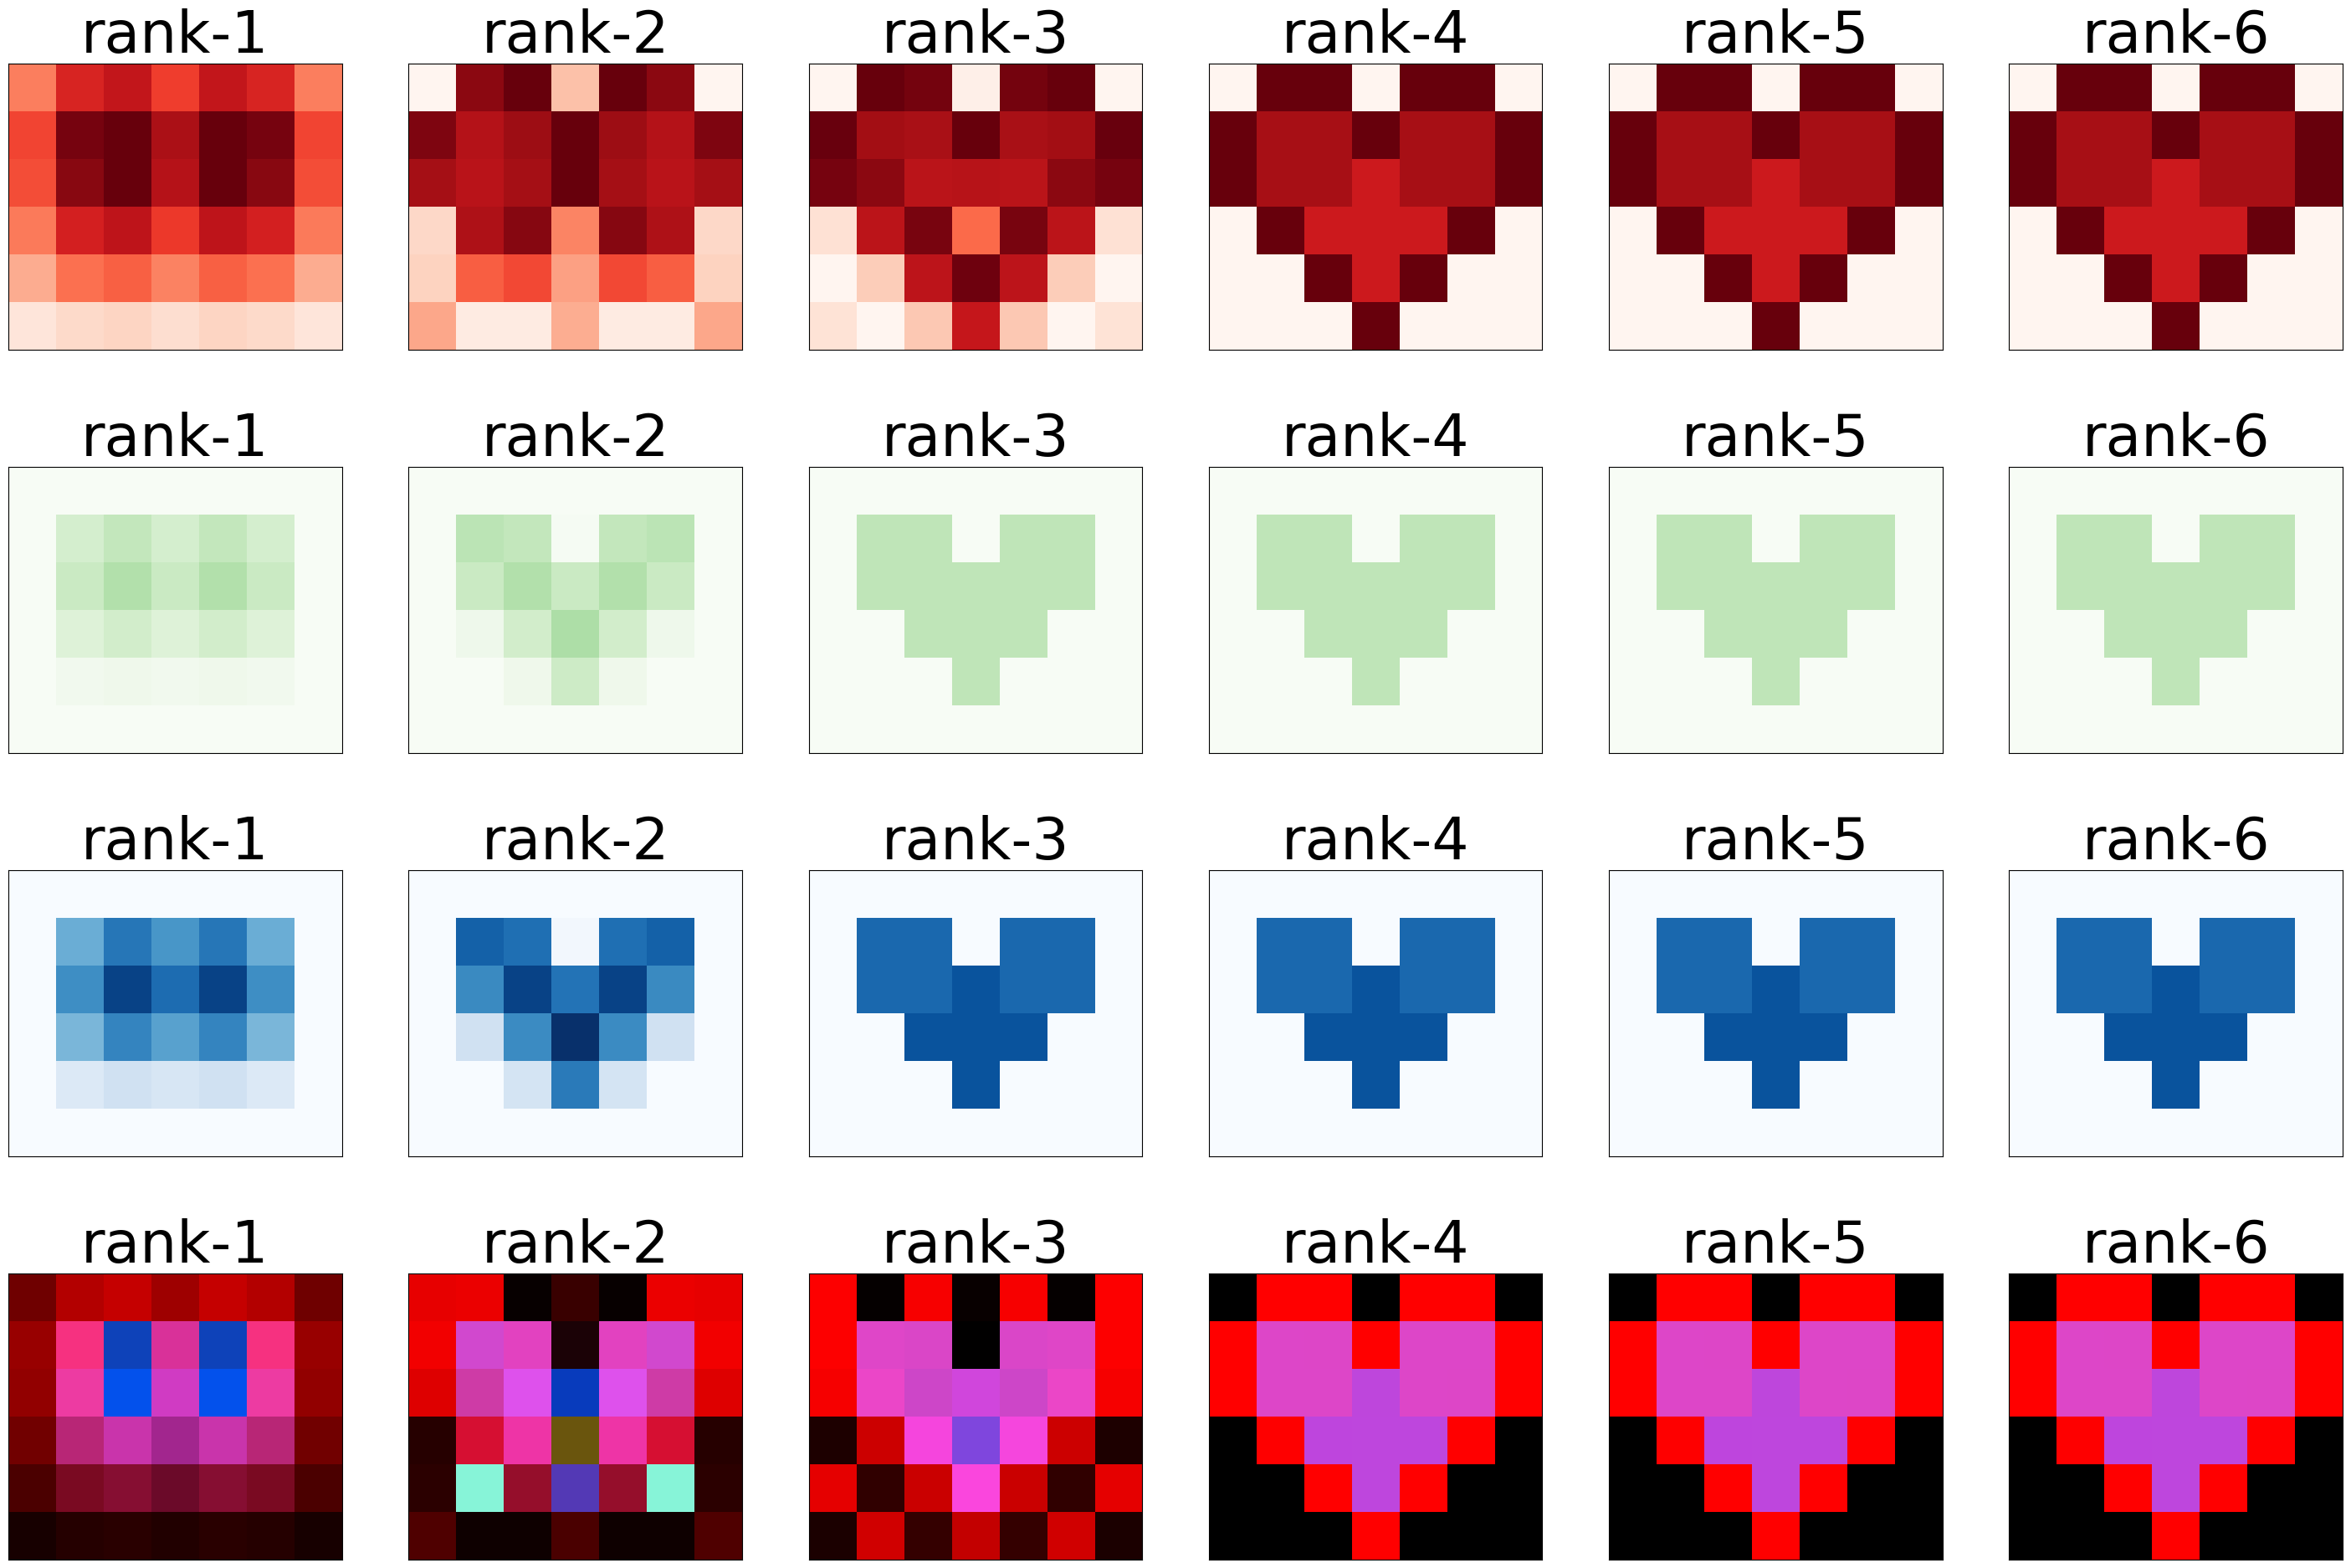
\includegraphics[width=0.61\linewidth]{img/colorheart.png}
        \caption{Rank-$k$ approximations of $R, G, B$ and their image}
        \label{fig:heartcolor}
    \end{figure}
\end{example}
\begin{example}
    To conclude, we will perform rank-$k$ approximations on our friend Mr. E. Paterno from earlier (\ref{fig:rgbarray}). Recall the $551 \times 693$ dimensions of each matrix of rank 551 and how they can be decomposed as a sum of 551 matrices.
    \begin{figure}
        \centering
        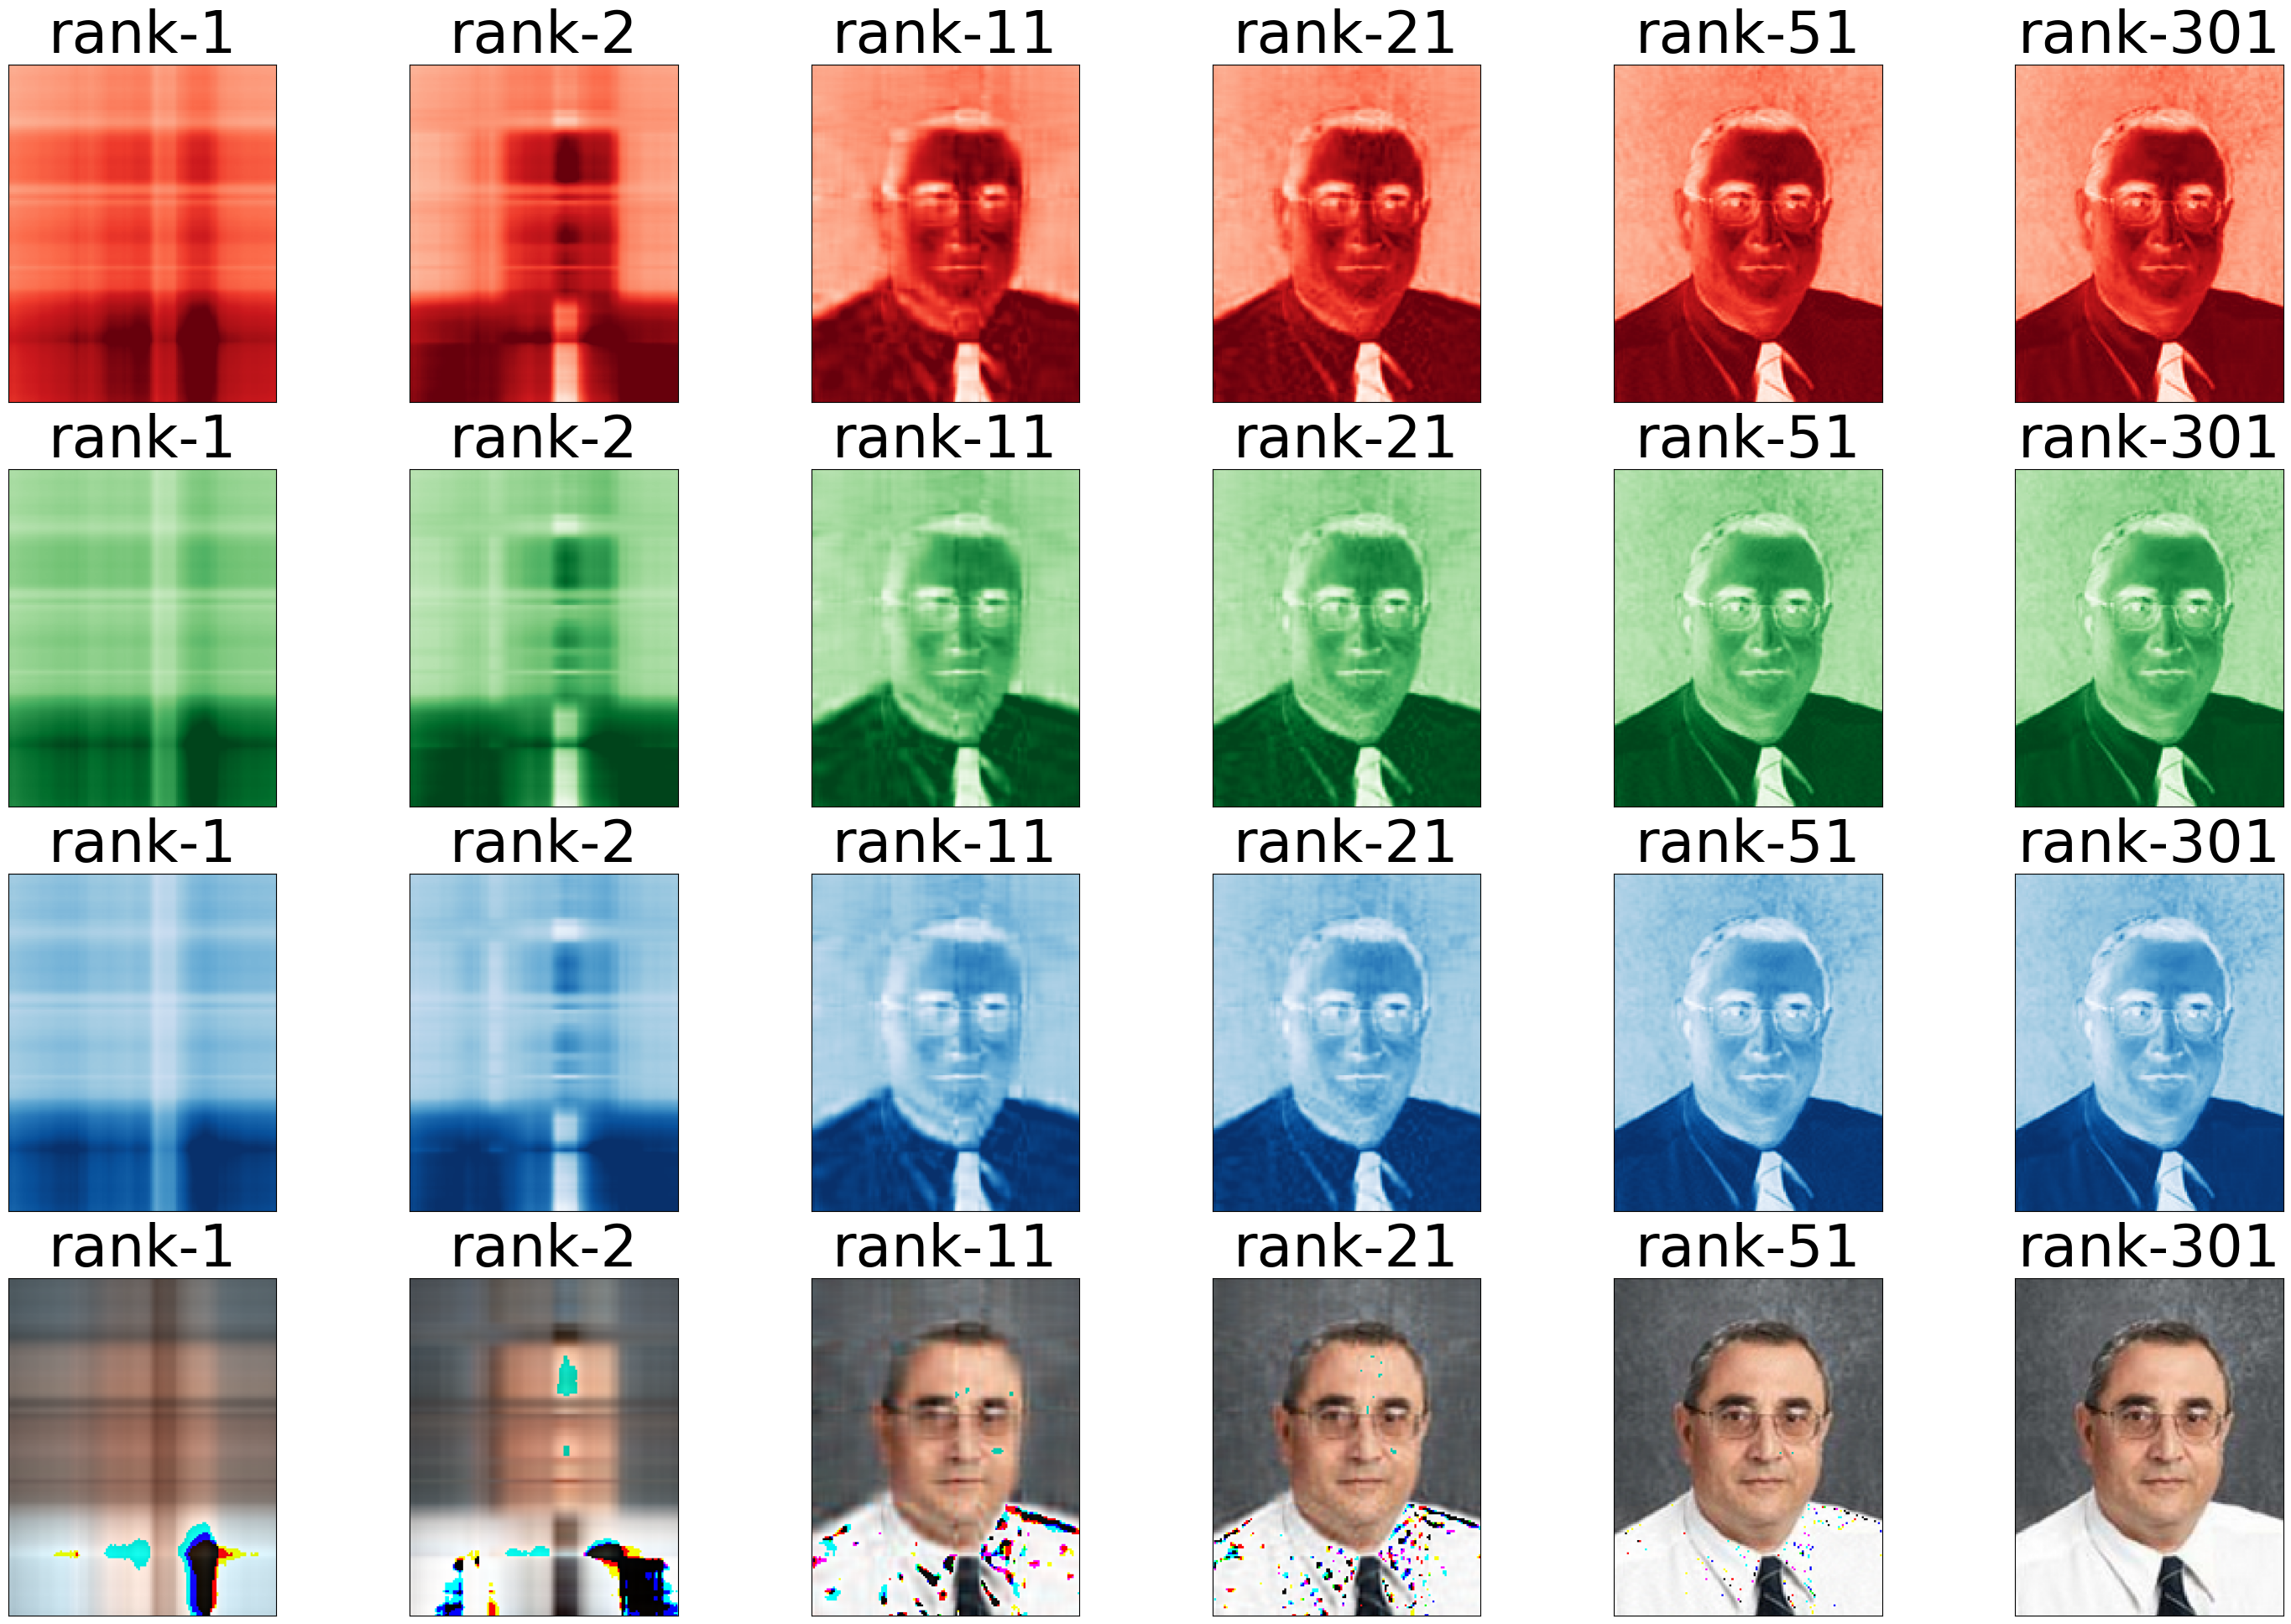
\includegraphics[width=0.7\linewidth]{img/paternoapproximation.png}
        \caption{Rank-$k$ approximations of Mr. E. Paterno's portrait}
        \label{fig:paternocolor}
    \end{figure}\\\\
    This enables a rank-$k$ approximation for each matrix, displayed in Figure \ref{fig:paternocolor}. Combining these approximations creates a rank-$k$ approximation for the original image. Observing this example reveals how rank-$k$ approximations approach the likeness of the original image as $k$ approaches $r$.
\end{example}
\section{Conclusion}
\noindent Modeling digital images as matrices allows us to reach into our linear algebra toolbox when faced with the task of processing images. With the ever-increasing demand for speed and efficiency, our newest tool, singular value decomposition, asserts itself as one of the most useful concepts in applied mathematics. Applicable to all matrices, SVD allows for the factorization and approximation of any digital image. This approximation, known as image compression, allows for images to be stored using less space while retaining their most important features. In the Information Age, where data powers every facet of life, linear algebra invites us to gain a deeper understanding of how information is transmitted and represented. As such, it can be a lifesaver…and a spacesaver?
\\
\\
\noindent \textbf{Acknowledgement.} The authors would like to thank Mr. Amro Mosaad, the \textit{Honors Linear Algebra} instructor at the Edison Academy, for guiding them through the fundamentals, applications, and extensions of linear algebra throughout the first semester.

\bibliographystyle{amsplain}
\begin{thebibliography}{99}

\bibitem{Compton} Compton, E. A. \& Ernstberger, L. Singular Value Decomposition: Applications to Image Processing. \textit{Citations Journal of Undergraduate Research}, 17, 101-105. \url{https://www.lagrange.edu/academics/undergraduate/undergraduate-research/citations/18-Citations2020.Compton.pdf}

\bibitem{Lay} Lay, D. C. (2012). Linear Algebra and Its Applications (4th ed.). \textit{Sections 2.9, 6.1, 6.2, 6.4, 7.1, 7.4} Addison-Wesley.

\bibitem{Weisstein} Weisstein, E. W. (2004, April 8). \textit{Conjugate Transpose}. Wolfram MathWorld. \url{https://mathworld.wolfram.com/ConjugateTranspose.html}

\bibitem{Fitzpatrick} Fitzpatrick, B. D. (2024, January 4). \textit{SVD} [PowerPoint slides]. Duke University.\\
\url{https://gitlab.oit.duke.edu/bdf10/218-lessons/-/raw/master/svd/svd.pdf}

\bibitem{Serrano} Serrano, L. [Serrano.Academy] (2020, September 3). \textit{Singular Value Decomposition (SVD) and Image Compression} [Video]. YouTube.
\url{https://www.youtube.com/watch?v=DG7YTlGnCEo}

\bibitem{Lakhotia} Lakhotia, Y. \& Pajaro, E. (2024). SVD Image Processing [Source code].
\url{https://github.com/yuviji/svd-image-processing}

\bibitem{Zelazko} Zelako, A. (2022). RGB colour model. In \textit{Encyclopædia Britannica}. Britannica.
\url{https://www.britannica.com/science/RGB-colour-model}

\bibitem{Devi} Devi, M. D. \& Sushma, G. S. N. (2022). Linear Algebra in Image Processing. \textit{Journal of Emerging Technologies and Innovative Research}, 9(4), 51-56.
\url{https://www.jetir.org/papers/JETIR2204008.pdf}

\bibitem{BBC} BBC. (2023). How do digital images work?. \textit{Bitesize, British Broadcasting Company}.
\url{https://www.bbc.co.uk/bitesize/articles/z2tgr82}

\end{thebibliography}

\end{document}

%------------------------------------------------------------------------------
% End of journal.tex
%------------------------------------------------------------------------------
